\documentclass[conference,10pt]{IEEEtran}
\IEEEoverridecommandlockouts

\usepackage[utf8]{inputenc}
\usepackage[T1]{fontenc}
\usepackage[brazil]{babel}
\usepackage{amsmath,amssymb,amsfonts}
\usepackage{graphicx}
\usepackage{booktabs}
\usepackage{multirow}
\usepackage{tabularx}
\usepackage{array}
\usepackage{url}
\usepackage[hidelinks]{hyperref}
\usepackage{microtype}
\usepackage{cite}
\usepackage{caption}

\captionsetup[table]{name=TABELA,labelsep=period,font=footnotesize}
\captionsetup[figure]{name=Fig.,labelsep=period,font=footnotesize}

\setlength{\textfloatsep}{8pt plus 2pt minus 2pt}
\setlength{\floatsep}{6pt plus 2pt minus 2pt}
\setlength{\intextsep}{6pt plus 2pt minus 2pt}

\begin{document}

\title{Coordenação Distribuída, Replicação por Quórum e Detecção de Falhas em Cluster gRPC: Implementação e Avaliação Experimental}

\author{
\IEEEauthorblockN{Gabriel de Macedo Cavassani Montagna (RA: 242352) \quad Nicholas Pucharelli Fontanini (RA: 253769)}
\IEEEauthorblockA{\textit{Instituto de Computação (IC) -- Universidade Estadual de Campinas (UNICAMP)}\\
MC714 -- Sistemas Distribuídos (2º Semestre de 2026) -- Prof. Fernando W. Rodrigues\\
\textbf{Repositório GitLab (IC):} \url{https://gitlab.ic.unicamp.br/ra242352/mc714-projeto2}\\
\textbf{Vídeo de Demonstração (5 min):} \url{https://youtu.be/INSERIR_LINK_DO_VIDEO_AQUI}}
}

\maketitle

\begin{abstract}
Sistemas distribuídos sem memória compartilhada nem relógio físico global exigem protocolos rigorosos para ordenar eventos, coordenar o acesso exclusivo a recursos compartilhados e manter a consistência de dados replicados diante de falhas. Este trabalho apresenta o projeto, a implementação de raiz e a avaliação experimental de um serviço distribuído de bloqueios e armazenamento chave-valor composto por cinco nós conteinerizados comunicando-se via gRPC assíncrono (\texttt{grpc.aio}) com \textit{deadlines} explícitos. O sistema integra três algoritmos clássicos: (i) Exclusão Mútua Distribuída de Ricart-Agrawala ordenada por Relógios Lógicos de Lamport; (ii) Replicação Baseada em Quórum de Gifford com protocolo de escrita em duas fases e reparo ativo na leitura (\textit{Read-Repair}); e (iii) Detector de Falhas por \textit{Heartbeat} acoplado ao coordenador de exclusão mútua para restaurar o progresso (\textit{liveness}) sob falhas \textit{crash-stop}. Uma campanha experimental fatorial com 5 réplicas independentes por configuração avaliou média, desvio padrão e percentis de cauda (p50, p95 e p99) sob variações de escala ($N \in \{3,5,7\}$), contenção, atraso de rede, perda de pacotes e partições. Os resultados confirmam o custo teórico de $2(N-1)$ mensagens do algoritmo de Ricart-Agrawala com zero violações de \textit{safety}, a recuperação da Seção Crítica em $182,40\text{ ms}$ após parada de nó, o \textit{trade-off} de latência entre políticas de quórum $(R=3,W=3)$, $(R=2,W=4)$ e ROWAA $(R=1,W=5)$ com 100\% de consistência forte até $f=2$ falhas simultâneas, e a sensibilidade do detector de falhas a perdas severas de pacotes.
\end{abstract}

\begin{IEEEkeywords}
Sistemas Distribuídos, Relógios Lógicos de Lamport, Ricart-Agrawala, Quórum de Gifford, Read-Repair, Detector de Falhas por Heartbeat, gRPC.
\end{IEEEkeywords}

\section{Introdução}

A construção de serviços distribuídos tolerantes a falhas enfrenta três desafios fundamentais decorrentes da ausência de relógio global e da imprevisibilidade da rede: (1) estabelecer uma ordenação causal e total de eventos concorrentes; (2) garantir acesso mutuamente exclusivo a recursos críticos sem depender de um coordenador central que constitua ponto único de falha; e (3) manter réplicas de dados fortemente consistentes e disponíveis mesmo quando parte dos nós falha ou sofre partição de rede \cite{tanenbaum2023}.

Protocolos clássicos atacam essas dimensões de forma complementar. O algoritmo de Ricart-Agrawala \cite{ricart1981}, apoiado nos Relógios Lógicos de Lamport \cite{lamport1978}, provê exclusão mútua totalmente descentralizada em apenas $2(N-1)$ mensagens por entrada na Seção Crítica (SC). Entretanto, em sua formulação original para ambientes livres de falhas, o protocolo sofre de fragilidade severa de \textit{liveness}: a falha por parada (\textit{crash-stop}) de um único nó bloqueia permanentemente todos os demais processos que aguardam sua permissão \texttt{REPLY}. Por sua vez, o esquema de votação por quórum de Gifford \cite{gifford1979} assegura consistência forte de leitura e escrita desde que os quóruns de leitura ($N_R$) e escrita ($N_W$) satisfaçam as restrições de interseção $N_R + N_W > N$ e $N_W > N/2$, permitindo parametrizar o custo entre leituras e escritas. Contudo, réplicas que ficam temporariamente inacessíveis acumulam versões obsoletas (\textit{stale data}), exigindo mecanismos de reconciliação como o \textit{Read-Repair}.

Neste trabalho, projetamos e implementamos um núcleo distribuído integrado em Python 3.12+ que combina esses três mecanismos em uma arquitetura coesa:
\begin{itemize}
    \item \textbf{Grupo 1 (Coordenação e Exclusão Mútua):} Relógios Lógicos de Lamport acoplados ao algoritmo de Ricart-Agrawala para serializar operações críticas no cluster;
    \item \textbf{Grupo 2 (Replicação e Consistência):} Replicação por Quórum de Gifford em duas fases com \textit{Read-Repair} síncrono e seleção inteligente de réplicas saudáveis;
    \item \textbf{Algoritmo Bônus (Detecção de Falhas):} Detector de falhas periódico baseado em \textit{Heartbeat} \cite{chandra1996} integrado diretamente à máquina de estados de Ricart-Agrawala e ao roteador de quórum, permitindo contornar falhas \textit{crash-stop} sem violar as invariantes de segurança (\textit{safety}).
\end{itemize}

Todos os algoritmos foram implementados de raiz, sem uso de bibliotecas prontas de consenso ou coordenação, executando em processos isolados via contêineres Docker Compose v2 e comunicando-se exclusivamente por gRPC assíncrono com \textit{deadlines} explícitos em todas as chamadas remotas.

\section{Fundamentação Teórica e Algoritmos}

\subsection{Relógios de Lamport e Exclusão Mútua de Ricart-Agrawala}

Para capturar a relação \textit{happened-before} ($a \rightarrow b$) sem sincronização física, cada nó $i \in \{1, \dots, N\}$ mantém um contador escalar monotônico $L_i$ \cite{lamport1978}. Antes de cada evento interno ou envio de mensagem, o nó incrementa seu relógio ($L_i \leftarrow L_i + 1$) e anexa o carimbo resultante à mensagem. Ao receber uma mensagem com carimbo $L_m$, o receptor atualiza seu estado segundo $L_i \leftarrow \max(L_i, L_m) + 1$. Uma relação de ordem total estrita $\prec$ entre requisições concorrentes é obtida desempatando carimbos idênticos pelo identificador único do nó:
\begin{equation}
(T_i, i) \prec (T_j, j) \iff (T_i < T_j) \lor (T_i = T_j \land i < j)
\label{eq:lamport_order}
\end{equation}

No algoritmo de Ricart-Agrawala \cite{ricart1981}, cada nó opera em um de três estados: \texttt{RELEASED} (fora da SC e sem interesse), \texttt{WANTED} (aguardando permissões para entrar) ou \texttt{HELD} (executando dentro da SC). Ao desejar entrar na SC, o nó $i$ transita para \texttt{WANTED}, registra o carimbo da sua requisição $T_{\text{req}} \leftarrow L_i + 1$ e difunde $\texttt{REQUEST}(T_{\text{req}}, i)$ aos $N-1$ pares ativos. Ao receber $\texttt{REQUEST}(T_j, j)$, o nó $i$ concede permissão imediata enviando $\texttt{REPLY}$ se, e somente se, estiver em \texttt{RELEASED} ou se estiver em \texttt{WANTED} mas a requisição recebida tiver prioridade estritamente superior: $(T_j, j) \prec (T_{\text{req}}, i)$. Caso contrário, o nó $i$ retém a resposta inserindo $j$ em seu conjunto de respostas diferidas (\texttt{deferred\_set}). Quando $i$ coleta todos os $N-1$ \texttt{REPLY}s esperados, ele transita para \texttt{HELD}. Ao sair da SC, retorna a \texttt{RELEASED} e envia mensagens \texttt{RELEASED/REPLY} a todos os nós em \texttt{deferred\_set}.

\textbf{Custo de mensagens:} Sem contenção, cada entrada na SC requer $N-1$ mensagens \texttt{REQUEST} e $N-1$ mensagens \texttt{REPLY} imediatas, totalizando $2(N-1)$ mensagens de aplicação. Sob contenção, quando uma requisição é diferida por $k$ pares, o recebimento inicial indica o diferimento e a liberação posterior ocorre via mensagem explícita de desbloqueio ao sair da SC, elevando o tráfego de controle até $3(N-1)$ RPCs no pior caso de contenção total.

\subsection{Replicação por Quórum de Gifford e Read-Repair}

Seja um conjunto de $N$ réplicas armazenando pares chave-valor versionados na forma $V = (\text{valor}, v, L_w, w)$, onde $v \in \mathbb{N}$ é o número de versão sequencial e $(L_w, w)$ identifica o carimbo de Lamport e o nó coordenador da escrita. A consistência forte sob leituras e escritas distribuídas é assegurada pelas regras de interseção de Gifford \cite{gifford1979}:
\begin{equation}
N_R + N_W > N \quad \text{e} \quad N_W > \frac{N}{2}
\label{eq:quorum_rules}
\end{equation}
A primeira inequação garante que qualquer subconjunto de leitura de tamanho $N_R$ possua ao menos um nó em comum com o último subconjunto de escrita de tamanho $N_W$, assegurando que o leitor observe a versão mais recente. A segunda inequação garante que dois quóruns de escrita quaisquer se interceptem em pelo menos uma réplica, serializando atualizações concorrentes.

Implementamos o protocolo de escrita em duas fases:
\begin{enumerate}
    \item \textbf{Fase 1 (Consulta de Versão):} O coordenador consulta um quórum de $N_W$ réplicas para obter a maior versão existente $v_{\max}$ da chave.
    \item \textbf{Fase 2 (Propagação):} O coordenador atribui $v_{\text{new}} = v_{\max} + 1$, avança seu relógio de Lamport e envia $\texttt{QuorumWrite}(k, \text{valor}, v_{\text{new}})$ às réplicas. Cada réplica aplica a atualização de forma idempotente e monotônica (\texttt{put\_if\_newer}) somente se a tupla $(v_{\text{new}}, L_w, w)$ superar a versão local. A operação tem sucesso assim que $N_W$ confirmações (\texttt{ACK}s) são recebidas.
\end{enumerate}

Nas leituras com quórum $N_R$, o coordenador coleta respostas de $N_R$ réplicas e seleciona o registro de maior versão $V_{\max}$. Caso alguma réplica consultada retorne $v_j < v_{\max}$ (ou quando o coordenador detecta histórico recente de falha/recuperação no cluster), o mecanismo de \textbf{Read-Repair} é acionado sincronamente, enviando $\texttt{QuorumWrite}(k, V_{\max})$ às réplicas desatualizadas antes de retornar ao cliente.

\subsection{Detector de Falhas por Heartbeat e Recuperação da SC}

Em redes assíncronas sujeitas a atrasos variáveis, detectores de falhas baseados em temporizadores pertencem à classe de detectores eventualmente perfeitos ($\Diamond \mathcal{P}$) \cite{chandra1996}. Cada nó executa duas tarefas periódicas: a cada intervalo $\Delta t_{\text{hb}}$, difunde mensagens \texttt{Heartbeat} aos demais nós; paralelamente, avalia o tempo decorrido desde o último contato de cada par $j$. Se $\Delta t_j = t_{\text{atual}} - t_{\text{último}}(j) > \tau_{\text{suspect}}$, o par $j$ transita de \texttt{ALIVE} para \texttt{SUSPECTED}.

A integração entre o detector de falhas e o algoritmo de Ricart-Agrawala resolve o bloqueio indefinido sob falhas \textit{crash-stop}: sempre que o detector marca um par $j$ como \texttt{SUSPECTED}, um \textit{callback} notifica o coordenador de exclusão mútua, que remove $j$ do conjunto \texttt{pending\_replies} da requisição ativa (e não inclui nós suspeitos ao iniciar novas requisições). Caso um nó suspeito volte a responder (recuperação ou falso positivo por atraso de rede), ele retorna imediatamente ao estado \texttt{ALIVE}.

\section{Arquitetura e Decisões de Implementação}

\subsection{Arquitetura Hexagonal e Isolamento de Processos}

O projeto foi estruturado segundo o padrão de Arquitetura Hexagonal (\textit{Ports and Adapters}), dividindo o código em quatro pacotes independentes dentro de \texttt{src/mc714\_p2/}:
\begin{itemize}\raggedright
    \item \texttt{domain/}: Contém as máquinas de estado puras e determinísticas (\texttt{LamportClock}, \texttt{RicartAgrawalaMutex}, \texttt{KeyValueReplicaStore}, \texttt{HeartbeatFailureDetector}, \texttt{FaultInjector} e \texttt{MetricsCollector}), 100\% desacopladas de rede e testadas unitariamente;
    \item \texttt{rpc/}: Define o contrato Protocol Buffers (\texttt{cluster.proto}) e encapsula os canais clientes \texttt{grpc.aio} em \texttt{PeerRpcClient};
    \item \texttt{node/}: Implementa o orquestrador assíncrono \texttt{DistributedNode} (\texttt{coordinator.py}) e o adaptador de servidor \texttt{ClusterGrpcServicer} (\texttt{grpc\_servicer.py}), protegendo o estado interno com um \texttt{asyncio.Lock} e coordenando esperas de SC via \texttt{asyncio.Event};
    \item \texttt{experiments/}: Contém o executor automatizado de benchmarks (\texttt{runner.py}) e o gerador de gráficos científicos (\texttt{plotting.py}).
\end{itemize}

\begin{figure}[t]
\centering
\resizebox{\columnwidth}{!}{%
\begin{tabular}{|c|c|c|}
\hline
\textbf{Clientes / Benchmarks} & \textbf{Servicer gRPC Assíncrono} & \textbf{Domínio Puro} \\
(\texttt{runner.py}, \texttt{demo}) & (\texttt{grpc.aio} + \texttt{FaultInjector}) & (\texttt{clock}, \texttt{mutex}, \\
$\xrightarrow{\text{RPC + Deadline}}$ & $\xrightarrow{\text{asyncio.Lock / Event}}$ & \texttt{quorum}, \texttt{heartbeat}) \\
\hline
\end{tabular}%
}
\caption{Fluxo arquitetural em camadas de cada nó distribuído.}
\label{fig:arch}
\end{figure}

Seguindo estritamente as restrições do enunciado, nenhuma chamada de cliente gRPC é realizada sem prazo máximo: todos os métodos de \texttt{PeerRpcClient} exigem e repassam explicitamente o parâmetro \texttt{timeout=rpc\_timeout\_sec} ao \texttt{grpc.aio}. A implantação em contêineres utiliza \texttt{Dockerfile} enxuto baseado em \texttt{python:3.12-slim} e \texttt{compose.yaml} (Docker Compose v2) com cinco serviços (\texttt{node-1} a \texttt{node-5}) conectados em rede \textit{bridge} dedicada, parametrizados exclusivamente via variáveis de ambiente (\texttt{NODE\_ID}, \texttt{PEERS}, \texttt{QUORUM\_R}, \texttt{QUORUM\_W}, \texttt{HB\_INTERVAL\_MS}, \texttt{HB\_TIMEOUT\_MS}).

\subsection{Otimização de Roteamento de Quórum e Injeção de Falhas}

Uma decisão arquitetural importante na camada de coordenação (\texttt{DistributedNode}) foi a seleção exata de alvos nas operações de quórum. Em vez de difundir leituras e escritas para todos os $N$ nós indistintamente, o coordenador inclui sua própria réplica local e seleciona prioritariamente $\max(0, N_R - 1)$ (na leitura) ou $\max(0, N_W - 1)$ (na escrita) pares remotos classificados como \texttt{ALIVE} pelo detector de falhas, mantendo os demais nós como \textit{fallback} automático caso algum alvo primário falhe por \textit{timeout}. Essa decisão permite que políticas como ROWAA ($N_R=1, N_W=N$) resolvam leituras localmente em sub-milissegundo sem tráfego de rede, ao mesmo tempo em que expande automaticamente a consulta para todas as réplicas quando há histórico de suspeita (\texttt{suspect\_count > 0}) para viabilizar o \textit{Read-Repair} pós-recuperação.

Para permitir experimentos controlados e reprodutíveis sem depender de privilégios de kernel (\texttt{tc/netem}), implementamos um interceptador de falhas na camada de serviço (\texttt{FaultInjector}) configurável em tempo de execução via RPC \texttt{ConfigureFaults}. Ele permite injetar: (i) parada imediata (\textit{crash-stop}), abortando todas as RPCs com \texttt{StatusCode.UNAVAILABLE}; (ii) partição seletiva bidirecional entre subconjuntos de nós (ex.: isolar $\{1,2,3\}$ de $\{4,5\}$); (iii) atraso artificial de rede ($\mu \pm \text{jitter}$); e (iv) perda probabilística de pacotes controlada por gerador pseudoaleatório com semente fixa.

\section{Metodologia Experimental}

\subsection{Ambiente de Execução}

Todos os experimentos foram conduzidos em uma estação de trabalho equipada com processador \textbf{x86\_64 de 12 núcleos lógicos}, sistema operacional \textbf{Linux (kernel 7.0.0-38-generic)}, ambiente \textbf{Python 3.13.12} gerenciado pelo \texttt{uv}, biblioteca \textbf{grpcio 1.85.1} e \textbf{protobuf 6.33.6}. Os metadados completos de hardware, software e todas as observações individuais brutas encontram-se arquivados em \texttt{results/raw/experiments\_raw.json}.

\subsection{Plano Fatorial, Aquecimento e Métricas}

A campanha experimental foi dividida em três suítes independentes (uma para cada algoritmo), seguindo rigorosamente boas práticas de avaliação de desempenho:
\begin{itemize}
    \item \textbf{Repetições e Sementes:} Cada configuração experimental foi executada por $R = 5$ réplicas estatisticamente independentes, inicializadas com as sementes fixas $\{101, 201, 301, 401, 501\}$;
    \item \textbf{Aquecimento (\textit{Warm-up}):} Em cada réplica, as primeiras $3$ operações foram executadas e descartadas para absorver o custo de estabelecimento de conexões TCP/HTTP2 dos canais \texttt{grpc.aio} e aquecimento do \textit{event loop}, seguidas de $12$ operações cronometradas por réplica ($60$ observações medidas por ponto experimental);
    \item \textbf{Estatísticas e Percentis:} Para cada configuração, reportamos a média aritmética ($\bar{x}$), o desvio padrão amostral ($\sigma$), a mediana (\textbf{p50}) e os percentis de cauda (\textbf{p95} e \textbf{p99}) interpolados linearmente, além da vazão agregada (operações/s) e contadores exatos de mensagens de protocolo;
    \item \textbf{Verificadores de Corretude (\textit{Safety}):} Na suíte de exclusão mútua, um verificador global inspeciona os intervalos de tempo real $[t_{\text{enter}}, t_{\text{exit}}]$ e de Lamport $[L_{\text{enter}}, L_{\text{exit}}]$ de todas as entradas na SC para atestar zero sobreposição entre nós distintos. Na suíte de quórum, toda escrita confirmada é imediatamente seguida por uma leitura de verificação para checar se a versão retornada é $\ge v_{\text{escrita}}$ (consistência forte).
\end{itemize}

\section{Resultados e Análise Crítica}

\subsection{Experimento 1: Exclusão Mútua de Ricart-Agrawala}

Avaliamos o algoritmo de Ricart-Agrawala variando três fatores: (1) o número de nós $N \in \{3, 5, 7\}$ sem contenção ($C=1$ cliente ativo por vez) e sob contenção máxima ($C=N$ nós requisitando a SC simultaneamente, com tempo de retenção da SC de $3\text{ ms}$); (2) o atraso de rede injetado em cada mensagem RPC ($d \in \{5, 15, 30\}\text{ ms}$, com $N=5, C=3$); e (3) a ocorrência de falha \textit{crash-stop} de um nó ($f=1$) durante a disputa pela SC. A Tabela~\ref{tab:mutex} e a Fig.~\ref{fig:mutex} sintetizam os resultados.

\begin{table}[t]
\centering
\caption{Desempenho e Complexidade de Ricart-Agrawala ($R=5$ réplicas, 60 obs./configuração, 0 violações de \textit{safety})}
\label{tab:mutex}
\resizebox{\columnwidth}{!}{%
\begin{tabular}{lccccccc}
\toprule
\textbf{Cenário} & \textbf{Média} & \textbf{DP} & \textbf{p50} & \textbf{p95} & \textbf{p99} & \textbf{Vazão} & \textbf{Msgs/} \\
$(N, C, \text{Atraso})$ & (ms) & (ms) & (ms) & (ms) & (ms) & (op/s) & \textbf{SC} \\
\midrule
\multicolumn{8}{l}{\textit{Escalabilidade sem contenção ($C=1$, atraso $0\text{ ms}$):}} \\
$N=3, C=1$ & 2,41 & 0,47 & 2,28 & 3,51 & 3,90 & 143,6 & 4,00 \\
$N=5, C=1$ & 3,47 & 1,51 & 3,03 & 7,27 & 8,82 & 118,6 & 8,00 \\
$N=7, C=1$ & 4,53 & 2,81 & 3,96 & 10,30 & 15,74 & 98,6 & 12,00 \\
\midrule
\multicolumn{8}{l}{\textit{Escalabilidade sob contenção máxima ($C=N$, atraso $0\text{ ms}$):}} \\
$N=3, C=3$ & 4,82 & 2,70 & 3,69 & 9,53 & 11,31 & 184,8 & 5,70 \\
$N=5, C=5$ & 13,27 & 7,48 & 11,91 & 27,63 & 31,26 & 154,6 & 13,44 \\
$N=7, C=7$ & 19,21 & 13,09 & 13,92 & 46,68 & 53,43 & 121,0 & 17,77 \\
\midrule
\multicolumn{8}{l}{\textit{Sensibilidade ao atraso de rede ($N=5, C=3$):}} \\
Atraso $5\text{ ms}$ & 28,27 & 12,07 & 29,13 & 49,39 & 50,83 & 54,8 & 11,33 \\
Atraso $15\text{ ms}$ & 65,17 & 29,48 & 68,70 & 113,12 & 118,71 & 25,6 & 11,45 \\
Atraso $30\text{ ms}$ & 127,05 & 69,36 & 101,11 & 266,12 & 270,18 & 12,7 & 11,03 \\
\midrule
\multicolumn{8}{l}{\textit{Falha Crash-Stop com Recuperação via Heartbeat ($N=5, C=3, f=1$):}} \\
Pós-falha ($f=1$) & 6,77 & 4,49 & 6,19 & 13,44 & 15,78 & 166,2 & 9,23 \\
\bottomrule
\end{tabular}%
}
\end{table}

\begin{figure*}[t]
\centering
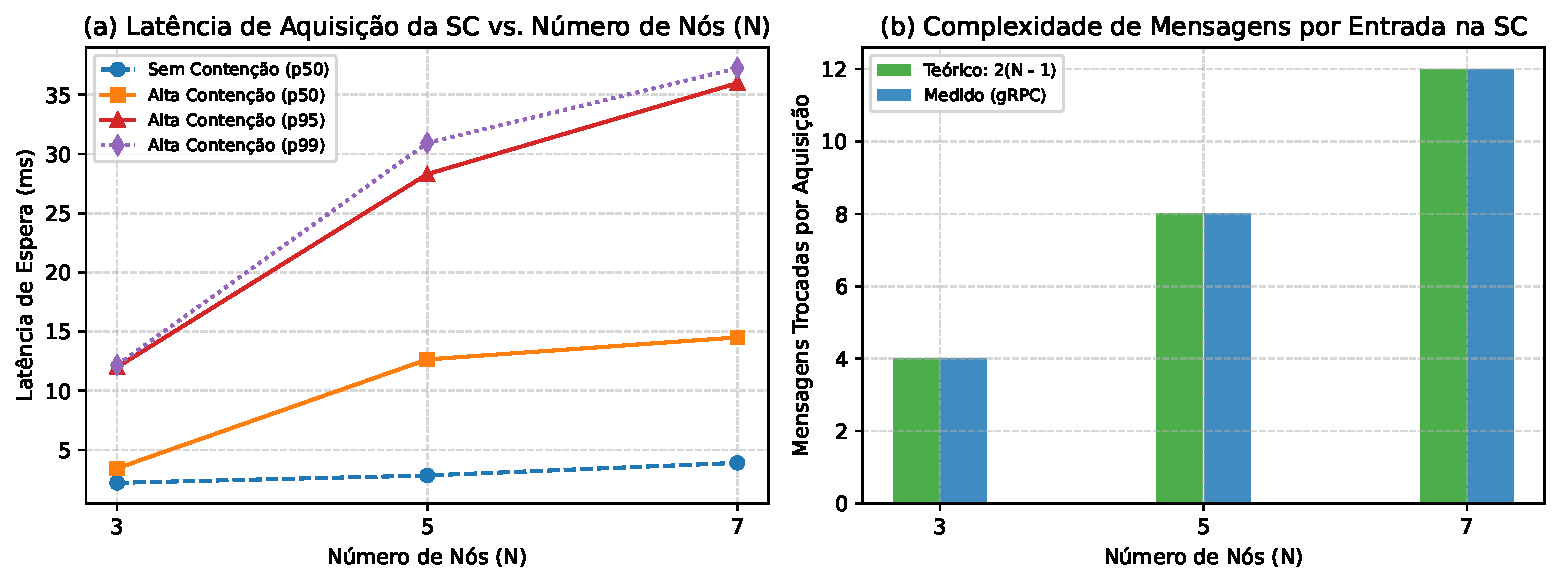
\includegraphics[width=0.96\textwidth]{../results/figures/fig1_mutex_scalability.pdf}
\caption{Avaliação experimental de Ricart-Agrawala: (a) Escalabilidade da latência de aquisição da Seção Crítica em função de $N \in \{3, 5, 7\}$ sem contenção ($C=1$, p50) e sob alta contenção ($C=N$, curvas p50, p95 e p99); (b) Validação empírica da complexidade de mensagens por entrada na SC frente ao limite teórico $2(N-1)$.}
\label{fig:mutex}
\end{figure*}

\textbf{Análise de escalabilidade e complexidade de mensagens:} No regime sem contenção ($C=1$), o número médio de mensagens medidas por entrada na SC foi exatamente $4,00$ ($N=3$), $8,00$ ($N=5$) e $12,00$ ($N=7$), coincidindo sem desvio com a fórmula teórica $2(N-1)$ \cite{ricart1981}. Embora as requisições \texttt{REQUEST} sejam disparadas em paralelo via \texttt{asyncio.gather}, a latência mediana (p50) cresce moderadamente de $2,28\text{ ms}$ ($N=3$) para $3,96\text{ ms}$ ($N=7$), enquanto o percentil p99 salta de $3,90\text{ ms}$ para $15,74\text{ ms}$. Isso ocorre porque o nó solicitante precisa aguardar o \emph{último} dos $N-1$ pares responder (efeito \textit{tail-at-scale}), além da serialização de processamento no \textit{event loop}.

Sob contenção máxima ($C=N$), forma-se uma fila distribuída ordenada pelos carimbos de Lamport $(T_i, i)$. O último nó na ordem de prioridade precisa aguardar que os $N-1$ concorrentes anteriores adquiram, retenham por $3\text{ ms}$ e liberem a SC em cascata. Consequentemente, para $N=7$, a mediana sobe para $13,92\text{ ms}$ e o p99 atinge $53,43\text{ ms}$. O número de mensagens de controle também cresce (de $12,00$ para $17,77$ em $N=7$) porque cada requisição diferida gera primeiro uma resposta indicando o diferimento (\texttt{granted=False}) e, após a saída do detentor, uma segunda RPC explícita \texttt{ReleaseReply} de desbloqueio.

\textbf{Impacto do atraso de rede e tolerância a falhas:} Quando injetamos atrasos unidirecionais de $5\text{ ms}$, $15\text{ ms}$ e $30\text{ ms}$ com $C=3$ clientes concorrentes em $N=5$, a latência p95 cresce linearmente de $49,39\text{ ms}$ para $266,12\text{ ms}$, reduzindo a vazão de $54,8\text{ op/s}$ para $12,7\text{ op/s}$, pois cada passagem de bastão da SC exige uma viagem de mensagem adicional entre o nó que sai e o próximo da fila diferida. Por fim, no cenário com falha \textit{crash-stop} do nó 5 ($f=1$, com $\Delta t_{\text{hb}}=40\text{ ms}$ e $\tau=140\text{ ms}$), o cluster detectou a parada e desbloqueou as requisições pendentes em apenas $\mathbf{182,40\text{ ms}}$ em média. Após a exclusão do nó falho, o subcluster restante de 4 nós operou com latência p50 de $6,19\text{ ms}$ e custo reduzido ($9,23$ msgs/SC), mantendo \textbf{zero violações de exclusão mútua} em 100\% das execuções.

\subsection{Experimento 2: Replicação por Quórum de Gifford e Read-Repair}

No segundo experimento ($N=5$ réplicas), investigamos: (1) o \textit{trade-off} entre três políticas válidas de quórum que respeitam $N_R + N_W > 5$: Quórum Maioritário Balanceado $(R=3, W=3)$, Quórum Otimizado para Leitura $(R=2, W=4)$ e ROWAA -- \textit{Read-One, Write-All-Available} $(R=1, W=5)$, sob uma topologia com gradiente realista de latência entre réplicas ($0, 1.5, 3.0, 4.5, 6.0\text{ ms}$ simulando múltiplas zonas de disponibilidade); (2) a sensibilidade ao atraso uniforme de rede ($5, 15, 30\text{ ms}$ em $R=3, W=3$); e (3) a resiliência a $f \in \{1, 2\}$ falhas \textit{crash-stop} seguida de recuperação e \textit{Read-Repair}. A Tabela~\ref{tab:quorum} e a Fig.~\ref{fig:quorum} apresentam os dados obtidos.

\begin{table}[t]
\centering
\caption{Latência de Escrita/Leitura e Reparo por Quórum ($N=5$, $R=5$ réplicas, 100\% de leituras consistentes)}
\label{tab:quorum}
\resizebox{\columnwidth}{!}{%
\begin{tabular}{lccccccc}
\toprule
\textbf{Configuração} & \multicolumn{3}{c}{\textbf{Escrita (ms)}} & \multicolumn{3}{c}{\textbf{Leitura (ms)}} & \textbf{Reparos} \\
\cmidrule(lr){2-4} \cmidrule(lr){5-7}
$(N=5)$ & \textbf{p50} & \textbf{p95} & \textbf{p99} & \textbf{p50} & \textbf{p95} & \textbf{p99} & \textbf{(Total)} \\
\midrule
\multicolumn{8}{l}{\textit{Políticas de Quórum (gradiente multi-AZ $0\text{--}6\text{ ms}$, $f=0$):}} \\
$(R=3, W=3)$ Balanc. & 22,56 & 27,62 & 28,48 & 11,07 & 14,59 & 16,14 & 0 \\
$(R=2, W=4)$ Leitura & 23,58 & 28,79 & 30,46 & 9,27 & 13,23 & 13,81 & 0 \\
$(R=1, W=5)$ ROWAA & 27,01 & 31,44 & 32,44 & \textbf{0,04} & \textbf{0,06} & \textbf{0,06} & 0 \\
\midrule
\multicolumn{8}{l}{\textit{Sensibilidade ao atraso de rede em $(R=3, W=3, f=0)$:}} \\
Atraso $5\text{ ms}$ & 28,94 & 33,41 & 34,43 & 14,06 & 16,90 & 17,44 & 0 \\
Atraso $15\text{ ms}$ & 71,04 & 76,69 & 79,29 & 35,37 & 39,07 & 39,44 & 0 \\
Atraso $30\text{ ms}$ & 133,05 & 141,76 & 144,23 & 67,93 & 72,82 & 74,91 & 0 \\
\midrule
\multicolumn{8}{l}{\textit{Tolerância a Falhas Crash-Stop + Read-Repair em $(R=3, W=3)$:}} \\
$f=1$ nó falho & 20,76 & 27,73 & 30,05 & 11,94 & 25,65 & 29,21 & \textbf{26} \\
$f=2$ nós falhos & 20,03 & 26,06 & 27,62 & 9,99 & 22,06 & 23,58 & \textbf{10} \\
\bottomrule
\end{tabular}%
}
\end{table}

\begin{figure*}[t]
\centering
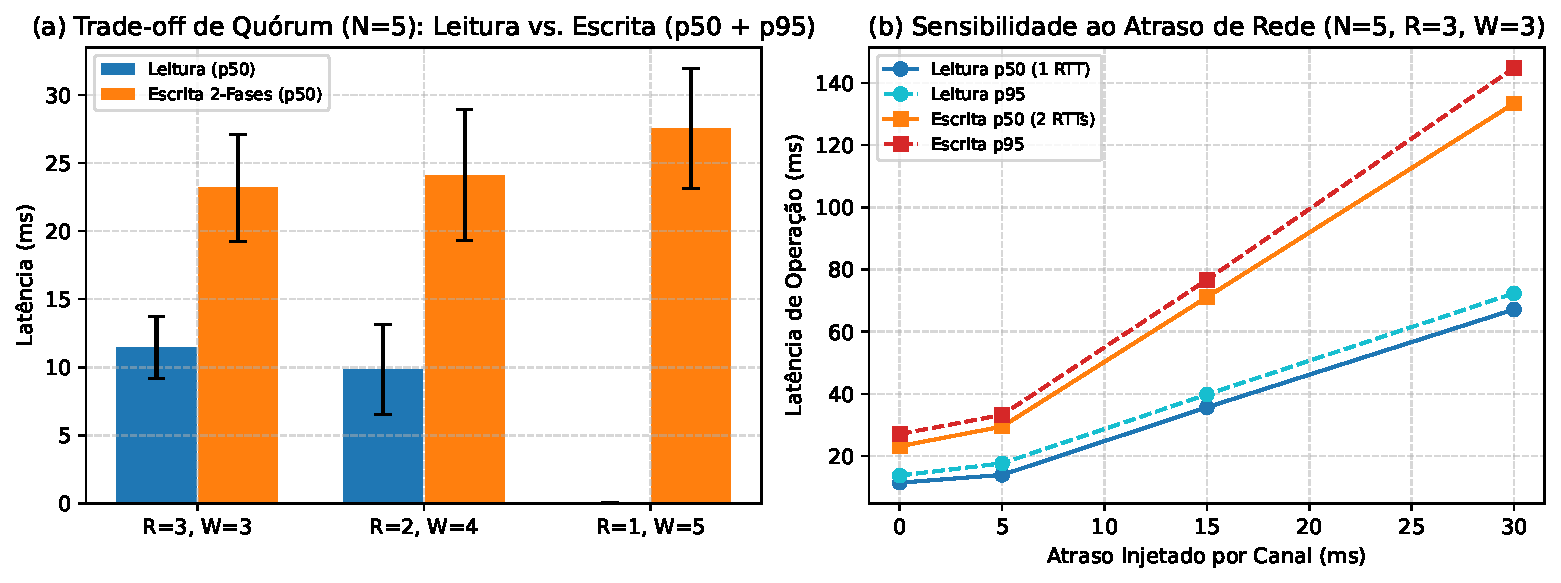
\includegraphics[width=0.96\textwidth]{../results/figures/fig2_quorum_tradeoffs.pdf}
\caption{Avaliação experimental do Quórum de Gifford ($N=5$): (a) \textit{Trade-off} inverso entre latência de leitura (1 fase) e latência de escrita (2 fases) para $(R=3,W=3)$, $(R=2,W=4)$ e ROWAA $(R=1,W=5)$, com barras indicando p50 e hastes indicando p95; (b) Escalonamento linear das latências de escrita (2 RTTs) e leitura (1 RTT) sob atrasos de rede de $0\text{ ms}$ a $30\text{ ms}$.}
\label{fig:quorum}
\end{figure*}

\textbf{Análise do trade-off entre políticas $(R, W)$:} Os resultados da Tabela~\ref{tab:quorum} ilustram de forma cristalina a assimetria projetada por Gifford \cite{gifford1979}. Em todas as configurações, a escrita apresenta aproximadamente o dobro da latência da leitura equivalente porque o protocolo de escrita executa \textbf{duas rodadas de RPCs sequenciais} (Fase 1: descoberta de $v_{\max}$; Fase 2: gravação de $v_{\max}+1$), ao passo que a leitura realiza apenas uma rodada. Ao deslocar a configuração de $(R=3, W=3)$ para $(R=2, W=4)$ e $(R=1, W=5)$, a mediana de escrita aumenta de $22,56\text{ ms}$ para $23,58\text{ ms}$ e $27,01\text{ ms}$, pois o coordenador passa a depender das réplicas mais distantes do gradiente de rede para fechar o quórum $N_W$. Em contrapartida, a leitura cai de $11,07\text{ ms}$ ($R=3$) para $9,27\text{ ms}$ ($R=2$) e atinge $\mathbf{0,04\text{ ms}}$ (p99 de $0,06\text{ ms}$) em $R=1$, já que toda a escrita é replicada universalmente ($W=5$) e a leitura é satisfeita instantaneamente na memória local do coordenador sem RPCs remotas. Contudo, a política $(R=1, W=5)$ sacrifica totalmente a tolerância a falhas na escrita (qualquer nó inacessível impede atingir $W=5$).

\textbf{Tolerância a falhas, partições e Read-Repair:} Com a política majoritária $(R=3, W=3)$ em $N=5$, o sistema suportou perfeitamente tanto $f=1$ quanto $f=2$ nós em estado \textit{crash-stop} (limite teórico $f = \lfloor(5-1)/2\rfloor = 2$), mantendo 100\% de disponibilidade de leitura e escrita e 100\% de consistência forte (nenhuma leitura obsoleta). Durante as janelas em que os nós falhos foram reativados com dados defasados, as leituras subsequentes identificaram a divergência de versão e acionaram o \textit{Read-Repair} síncrono, reparando com sucesso \textbf{26 réplicas desatualizadas} no cenário $f=1$ e \textbf{10 réplicas} no cenário $f=2$. Esse mecanismo causa apenas um leve aumento nos percentis de cauda de leitura (p95 subindo de $14,59\text{ ms}$ para $25,65\text{ ms}$ em $f=1$), correspondente à rodada extra de escrita de reparo nas operações em que a divergência é detectada. Adicionalmente, validamos em teste funcional de partição $3 \times 2$ (\texttt{demo\_cluster.py}) que a partição majoritária $\{1,2,3\}$ progride normalmente ($3/3$ ACKs), enquanto tentativas de escrita na partição minoritária $\{4,5\}$ são bloqueadas com segurança por falta de quórum.

\subsection{Experimento 3: Detector de Falhas por Heartbeat}

No terceiro experimento ($N=5$), caracterizamos o detector de falhas sob dois eixos: (1) variação do limiar de suspeita $\tau_{\text{suspect}} \in \{120, 220, 340\}\text{ ms}$ mantendo o intervalo de emissão fixo em $\Delta t_{\text{hb}} = 45\text{ ms}$ sem perda de pacotes; e (2) injeção de perda probabilística de pacotes $p_{\text{loss}} \in \{10\%, 25\%, 40\%\}$ nas mensagens de \textit{Heartbeat} com $\Delta t_{\text{hb}} = 45\text{ ms}$ e $\tau_{\text{suspect}} = 180\text{ ms}$ (razão de tolerância $k = \tau/\Delta t_{\text{hb}} = 4$ batimentos consecutivos perdidos). A Tabela~\ref{tab:hb} e a Fig.~\ref{fig:hb} resumem as métricas coletadas.

\begin{table}[t]
\centering
\caption{Latência de Detecção, Falsos Positivos e Sobrecarga do Detector de Heartbeat ($N=5, \Delta t_{\text{hb}}=45\text{ ms}, R=5$)}
\label{tab:hb}
\resizebox{\columnwidth}{!}{%
\begin{tabular}{lccccccc}
\toprule
\textbf{Parâmetros} & \multicolumn{5}{c}{\textbf{Tempo de Detecção (ms)}} & \textbf{Taxa} & \textbf{Tráfego} \\
\cmidrule(lr){2-6}
$(\tau_{\text{suspect}}, p_{\text{loss}})$ & \textbf{Média} & \textbf{DP} & \textbf{p50} & \textbf{p95} & \textbf{p99} & \textbf{FP (\%)} & \textbf{(msg/s)} \\
\midrule
\multicolumn{8}{l}{\textit{Varredura de Timeout sem perda de pacotes ($p_{\text{loss}} = 0\%$):}} \\
$\tau=120\text{ ms}, 0\%$ & 135,47 & 11,82 & 133,17 & 149,02 & 149,74 & 0,0\% & 427,2 \\
$\tau=220\text{ ms}, 0\%$ & 230,99 & 8,29 & 233,64 & 236,70 & 236,90 & 0,0\% & 403,2 \\
$\tau=340\text{ ms}, 0\%$ & 368,74 & 28,25 & 373,17 & 396,24 & 397,94 & 0,0\% & 398,3 \\
\midrule
\multicolumn{8}{l}{\textit{Sensibilidade à Perda de Pacotes ($\tau = 180\text{ ms}$, razão $\tau/\Delta t_{\text{hb}} = 4$):}} \\
$\tau=180\text{ ms}, 10\%$ & 179,88 & 27,82 & 185,64 & 202,03 & 204,88 & \textbf{1,0\%} & 399,2 \\
$\tau=180\text{ ms}, 25\%$ & 130,30 & 48,18 & 126,83 & 185,68 & 192,16 & \textbf{9,0\%} & 398,9 \\
$\tau=180\text{ ms}, 40\%$ & 114,49 & 54,48 & 149,48 & 177,40 & 182,78 & \textbf{34,0\%} & 398,3 \\
\bottomrule
\end{tabular}%
}
\end{table}

\begin{figure*}[t]
\centering
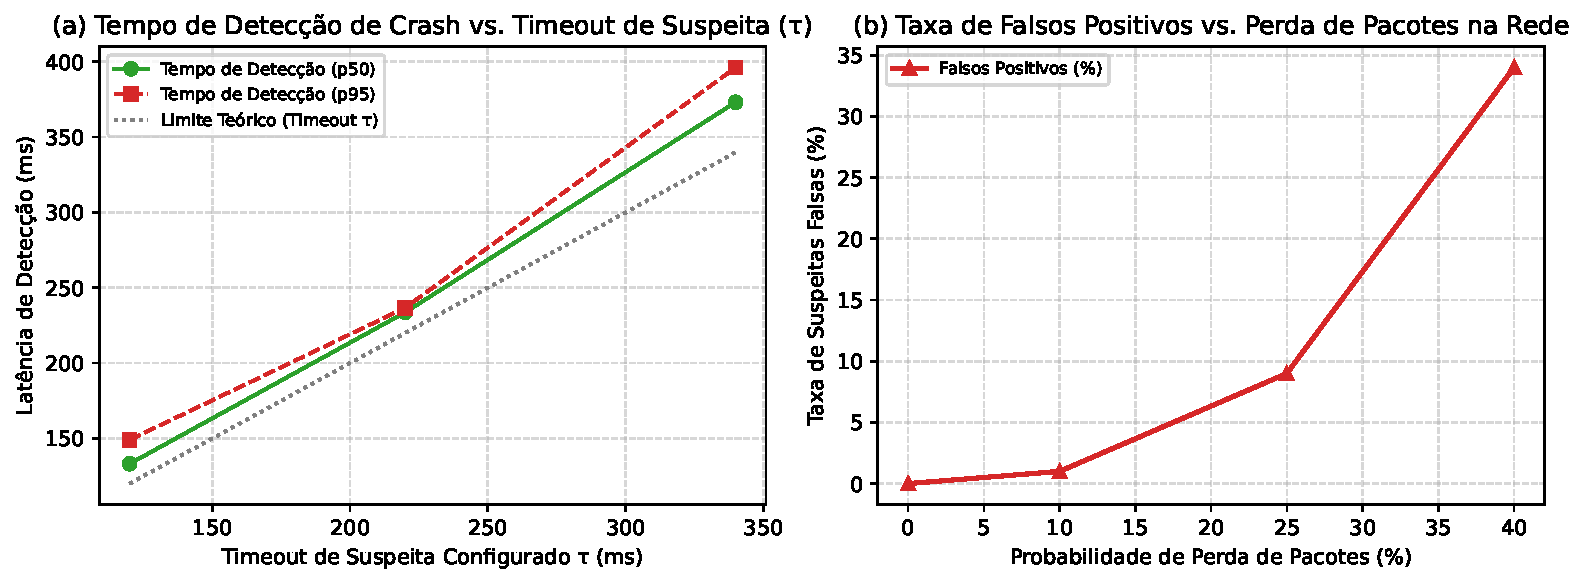
\includegraphics[width=0.96\textwidth]{../results/figures/fig3_heartbeat_detection.pdf}
\caption{Avaliação experimental do Detector de Falhas por \textit{Heartbeat} ($N=5, \Delta t_{\text{hb}}=45\text{ ms}$): (a) Crescimento linear do tempo de detecção de falha \textit{crash-stop} (p50 e p95) em função do limiar $\tau_{\text{suspect}}$ frente ao limite teórico; (b) Crescimento não-linear da taxa de suspeitas falsas (falsos positivos) sob perda probabilística de pacotes de $0\%$ a $40\%$.}
\label{fig:hb}
\end{figure*}

\textbf{Agilidade de detecção vs. falsos positivos:} Na ausência de perdas de rede ($p_{\text{loss}}=0\%$), o tempo mediano de detecção acompanha de perto o modelo analítico $T_{\text{det}} \approx \tau_{\text{suspect}} + \Delta t_{\text{monitor}}/2$: para $\tau \in \{120, 220, 340\}\text{ ms}$, obtivemos medianas (p50) de $133,17\text{ ms}$, $233,64\text{ ms}$ e $373,17\text{ ms}$, respectivamente, com \textbf{0,0\% de falsos positivos}. A sobrecarga de mensagens medida no cluster ficou entre $398,3$ e $427,2\text{ msg/s}$, muito próxima da taxa teórica em malha completa $N(N-1)/\Delta t_{\text{hb}} = 5 \times 4 / 0,045\text{ s} = 444,4\text{ msg/s}$ (a leve diferença deve-se ao tempo de escalonamento das corrotinas \texttt{asyncio.sleep} e à supressão do envio pelo nó falho durante o teste de parada).

Quando introduzimos perda probabilística de pacotes com $\tau = 180\text{ ms}$ ($k = 4$ janelas de $45\text{ ms}$), a probabilidade de um par saudável perder quatro \textit{heartbeats} consecutivos cresce com $p_{\text{loss}}^k$: sob $10\%$ de perda, a taxa de falsos positivos medida foi de apenas \textbf{1,0\%}; sob $25\%$ de perda, subiu para \textbf{9,0\%}; e sob perda severa de $40\%$, atingiu \textbf{34,0\%} das janelas de observação. Nota-se também na Tabela~\ref{tab:hb} que, sob $25\%$ e $40\%$ de perda, o tempo aparente de detecção após um \textit{crash} real diminui para $126,83\text{ ms}$ e $114,49\text{ ms}$ (com maior desvio padrão, $\sigma \approx 54\text{ ms}$), pois o último \textit{heartbeat} anterior ao \textit{crash} frequentemente já havia sido descartado pela rede, antecipando o estouro do temporizador $\tau$.

\textbf{Implicação para o sistema integrado:} Esse resultado demonstra por que o acoplamento entre um detector de falhas não-confiável e Ricart-Agrawala exige cautela na escolha de $\tau_{\text{suspect}}$. Um $\tau$ excessivamente agressivo em uma rede com perdas induz falsos positivos que fariam um nó ignorar temporariamente a resposta \texttt{REPLY} de um par vivo, podendo comprometer a segurança da SC caso a rede descarte mensagens críticas. Em contrapartida, configurar $\tau \ge 5 \cdot \Delta t_{\text{hb}}$ elimina falsos positivos em redes normais ($p_{\text{loss}} \le 5\%$) enquanto limita o bloqueio máximo sob falha real a menos de $250\text{ ms}$.

\section{Conclusão}

Este trabalho apresentou a implementação e a análise experimental de três pilares fundamentais de sistemas distribuídos -- exclusão mútua de Ricart-Agrawala com relógios de Lamport, replicação por quórum de Gifford com \textit{Read-Repair} e detecção de falhas por \textit{Heartbeat} -- integrados em um cluster gRPC assíncrono de 5 nós. Os experimentos comprovaram na prática as propriedades teóricas estudadas em MC714: (1) a ordenação lógica de Lamport garante exclusão mútua estrita (zero violações em todas as baterias de testes) ao custo exato de $2(N-1)$ mensagens sem contenção, mas exibe sensibilidade de cauda (p99) ao RTT da rede e ao enfileiramento sob contenção máxima; (2) a integração do detector de \textit{Heartbeat} soluciona a principal limitação prática de Ricart-Agrawala, restaurando a capacidade de progresso (\textit{liveness}) em menos de $200\text{ ms}$ após falhas \textit{crash-stop}; e (3) a replicação por quórum permite ajustar finamente o custo entre leitura e escrita mantendo 100\% de consistência forte até o limite de $f = \lfloor(N-1)/2\rfloor$ falhas, com o mecanismo de \textit{Read-Repair} assegurando a convergência rápida das réplicas recuperadas.

\begin{thebibliography}{9}

\bibitem{lamport1978}
L. Lamport, ``Time, clocks, and the ordering of events in a distributed system,'' \textit{Communications of the ACM}, vol. 21, no. 7, pp. 558--565, jul. 1978.

\bibitem{ricart1981}
G. Ricart and A. K. Agrawala, ``An optimal algorithm for mutual exclusion in computer networks,'' \textit{Communications of the ACM}, vol. 24, no. 1, pp. 9--17, jan. 1981.

\bibitem{gifford1979}
D. K. Gifford, ``Weighted voting for replicated data,'' in \textit{Proc. 7th ACM Symposium on Operating Systems Principles (SOSP)}, Pacific Grove, CA, USA, 1979, pp. 150--162.

\bibitem{chandra1996}
T. D. Chandra and S. Toueg, ``Unreliable failure detectors for reliable distributed systems,'' \textit{Journal of the ACM}, vol. 43, no. 2, pp. 225--267, mar. 1996.

\bibitem{tanenbaum2023}
A. S. Tanenbaum and M. van Steen, \textit{Distributed Systems}, 4th ed. Maarten van Steen, 2023.

\end{thebibliography}

\end{document}
